% =====================================================================
% Section: Multi-Agent for Monitoring, Diagnosing, Planning and Action
% Source: experiments/E-L2-MultiAgent_Pipeline/ (run_pipeline.py + visualize.py)
%
% This section is intended for inclusion in Chapter 5 (Layer 2 Agentic AI)
% as a sub-section after the V3 ensemble validation. It demonstrates an
% alternative deployment pattern: a sequential 4-stage role-specialised
% LLM pipeline (vs the parallel-vote ensemble used in E-L2 V3).
% =====================================================================

\section{Multi-Agent for Monitoring, Diagnosing, Planning and Action}

The E-L2 V3 evaluation (preceding section) demonstrates that a parallel 3-LLM majority-vote ensemble can assign machine-level criticality tiers with substantial agreement against composite ground truth. For deployment scenarios that require a richer structured-output trail --- including diagnostic root-cause identification, explicit maintenance action planning, and CMMS-compatible work-order dispatch --- this section presents an alternative \emph{sequential 4-stage agentic pipeline} where each stage is a role-specialised LLM and each stage's output feeds the next as structured JSON.

\subsection{Pipeline Architecture}

Figure~\ref{fig:multi_agent_pipeline} shows the 4-stage flow. Each stage receives a well-defined input, produces a well-defined JSON output, and hands off to the next stage:

\begin{enumerate}
    \item \textbf{Stage 1 --- Monitoring (\texttt{glm-5.1:cloud})}: receives Layer~1 evidence (5 sensor readings + upstream classifier outputs: failure\_type, anomaly\_flag, downtime\_risk, maintenance\_required, RUL forecast) and produces \texttt{\{status, severity, flagged\_sensors, reasoning, confidence\}}.
    \item \textbf{Stage 2 --- Diagnosing (\texttt{deepseek-v4-pro:cloud})}: receives the Monitoring output plus the original evidence and produces \texttt{\{root\_cause, affected\_component, failure\_progression, evidence, confidence\}} --- the diagnostic hypothesis.
    \item \textbf{Stage 3 --- Planning (\texttt{kimi-k2.6:cloud})}: receives the Diagnosing output and produces \texttt{\{action, priority, estimated\_duration\_hours, employees\_needed, skills\_needed, scheduled\_within\_hours, justification\}} --- the maintenance action plan.
    \item \textbf{Stage 4 --- Action (\texttt{deepseek-v4-pro:cloud})}: receives the Planning output and the machine identifier and produces \texttt{\{work\_order\_id, action\_type, dispatched\_to, scheduled\_time, approval\_required, status, audit\_note\}} --- the CMMS-style dispatch decision (with explicit human-in-the-loop approval gate for high-priority actions).
\end{enumerate}

\begin{figure}[htbp]
    \centering
    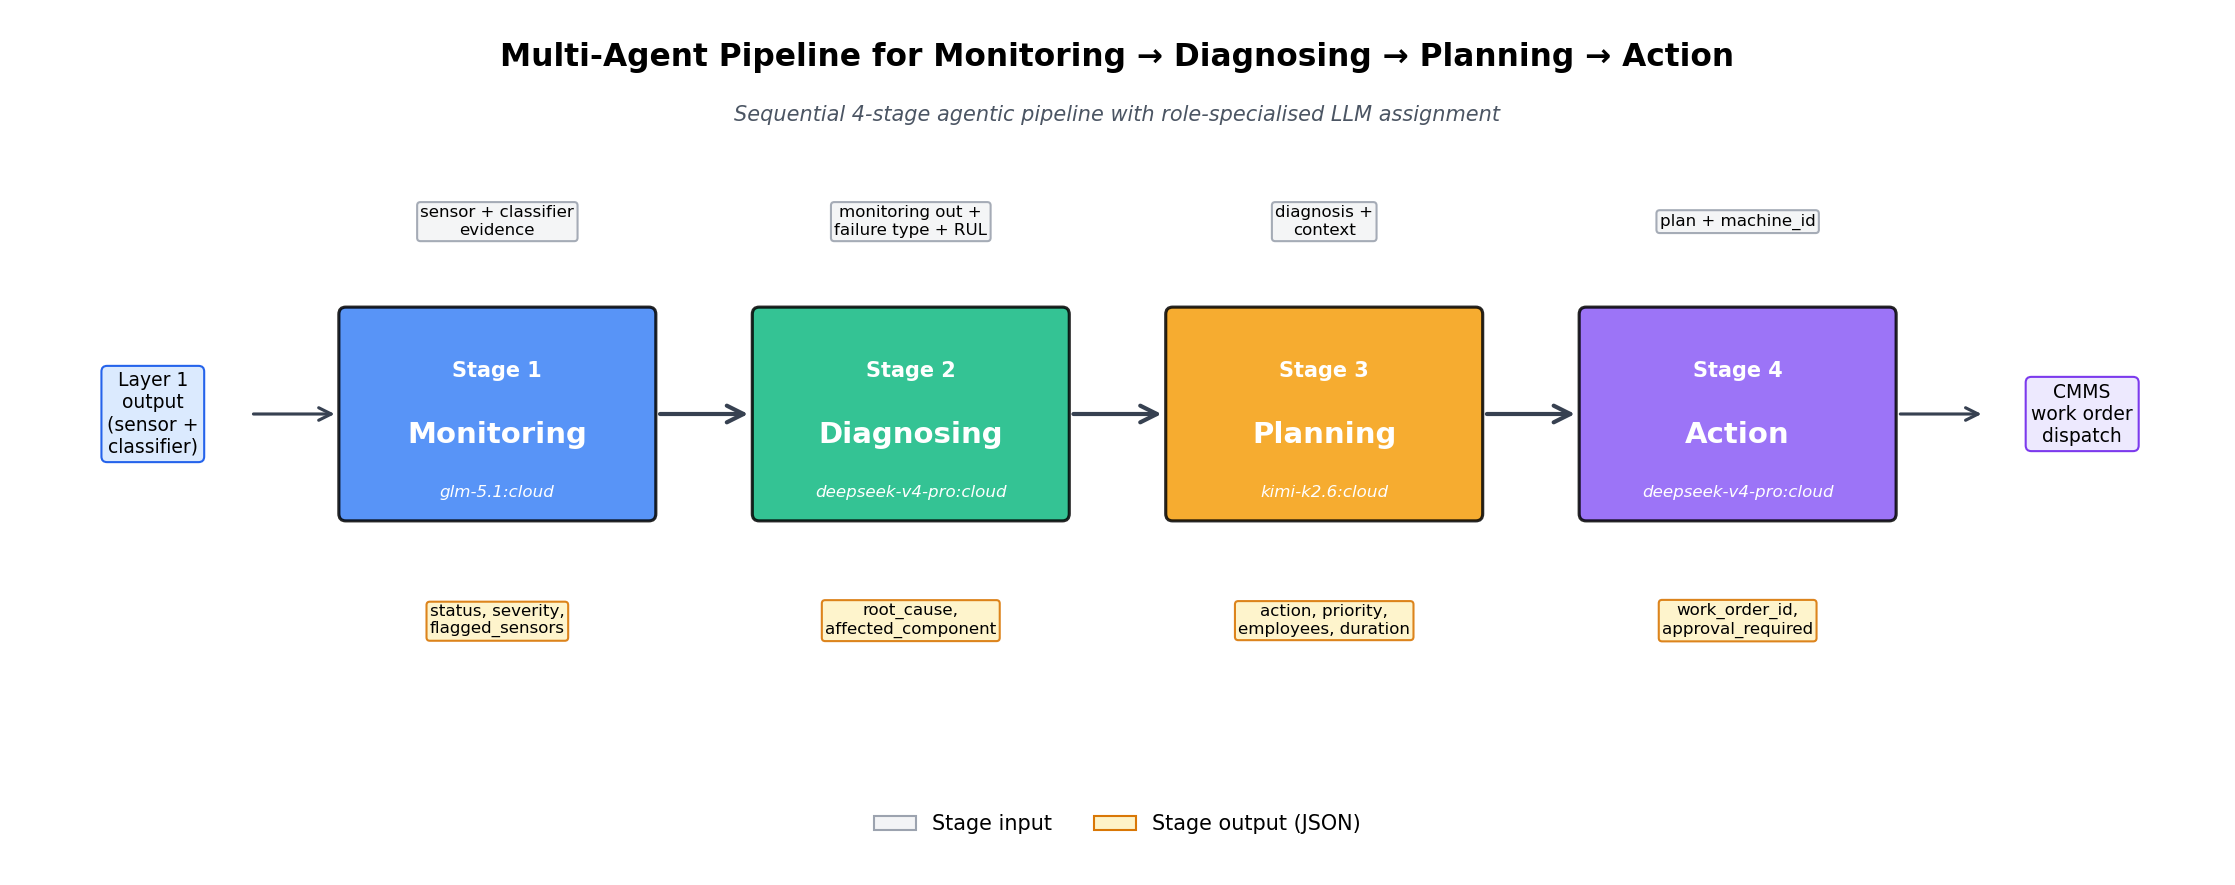
\includegraphics[width=\textwidth]{figures/pipeline_architecture.png}
    \caption{Multi-Agent Pipeline architecture. Layer~1 output feeds the Monitoring stage; each stage hands off a structured JSON object to the next. The final Action stage produces a CMMS-ready work-order dispatch decision with explicit approval-required flag for high-priority interventions. LLM assignment per stage is informed by the per-LLM ablation in E-L2 V3 (\texttt{deepseek-v4-pro:cloud} highest individual $\kappa = 0.728$, used for the two reasoning-heavy stages; \texttt{glm-5.1:cloud} fast pre-screen; \texttt{kimi-k2.6:cloud} structured-output generator).}
    \label{fig:multi_agent_pipeline}
\end{figure}

\subsection{Implementation}

The pipeline is implemented in \texttt{experiments/E-L2-MultiAgent\_Pipeline/run\_pipeline.py}. The relevant control flow is:

\begin{verbatim}
def run_pipeline_one(case):
    trace = {"machine_id": case["machine_id"], "stages": {}}

    # Stage 1: Monitoring
    p1 = prompt_monitoring(case)
    r1 = call_llm(AGENT_LLM["monitoring"], p1)
    j1 = extract_json(r1["content"])
    trace["stages"]["monitoring"] = {"parsed": j1, ...}
    if not j1: return trace  # halt on parse failure

    # Stage 2: Diagnosing
    p2 = prompt_diagnosing(case, j1)
    r2 = call_llm(AGENT_LLM["diagnosing"], p2)
    j2 = extract_json(r2["content"])
    trace["stages"]["diagnosing"] = {"parsed": j2, ...}
    if not j2: return trace

    # Stage 3: Planning
    p3 = prompt_planning(j2, case)
    r3 = call_llm(AGENT_LLM["planning"], p3)
    j3 = extract_json(r3["content"])
    trace["stages"]["planning"] = {"parsed": j3, ...}
    if not j3: return trace

    # Stage 4: Action
    p4 = prompt_action(j3, case["machine_id"])
    r4 = call_llm(AGENT_LLM["action"], p4)
    j4 = extract_json(r4["content"])
    trace["stages"]["action"] = {"parsed": j4, ...}

    return trace
\end{verbatim}

Each LLM call is cached to disk (keyed on \texttt{sha256(model + prompt)}), allowing fully deterministic replay of a recorded run without re-incurring API cost. JSON extraction is robust to common LLM output patterns (\texttt{```json} fences, trailing commas, leading/trailing prose).

\subsection{Demo Execution and Output}

The pipeline was executed on 5 demo machines drawn from the test split, intentionally spanning the four ground-truth criticality tiers (Critical, High, Medium, Low) for illustrative diversity. The complete trace is preserved at \texttt{experiments/E-L2-MultiAgent\_Pipeline/trace.json}; summary metrics are in \texttt{summary.csv}.

Table~\ref{tab:multi_agent_trace} (rendered as Figure~\ref{fig:multi_agent_trace}) shows the per-machine trace. All five pipelines completed all four stages without parse failure. The Monitoring stage classifies status as \texttt{warning} or \texttt{anomaly}; the Diagnosing stage identifies plausible root causes (cooling system inefficiency, seal degradation); the Planning stage proposes appropriate actions (\texttt{repair} for the Critical machine with P2 priority, \texttt{monitor} for the misclassified-as-normal High-tier machine, \texttt{replace}/\texttt{inspect} for Medium and Low tiers); the Action stage correctly routes only the P2 \texttt{repair} action to human approval and dispatches the lower-priority actions automatically.

\begin{figure}[htbp]
    \centering
    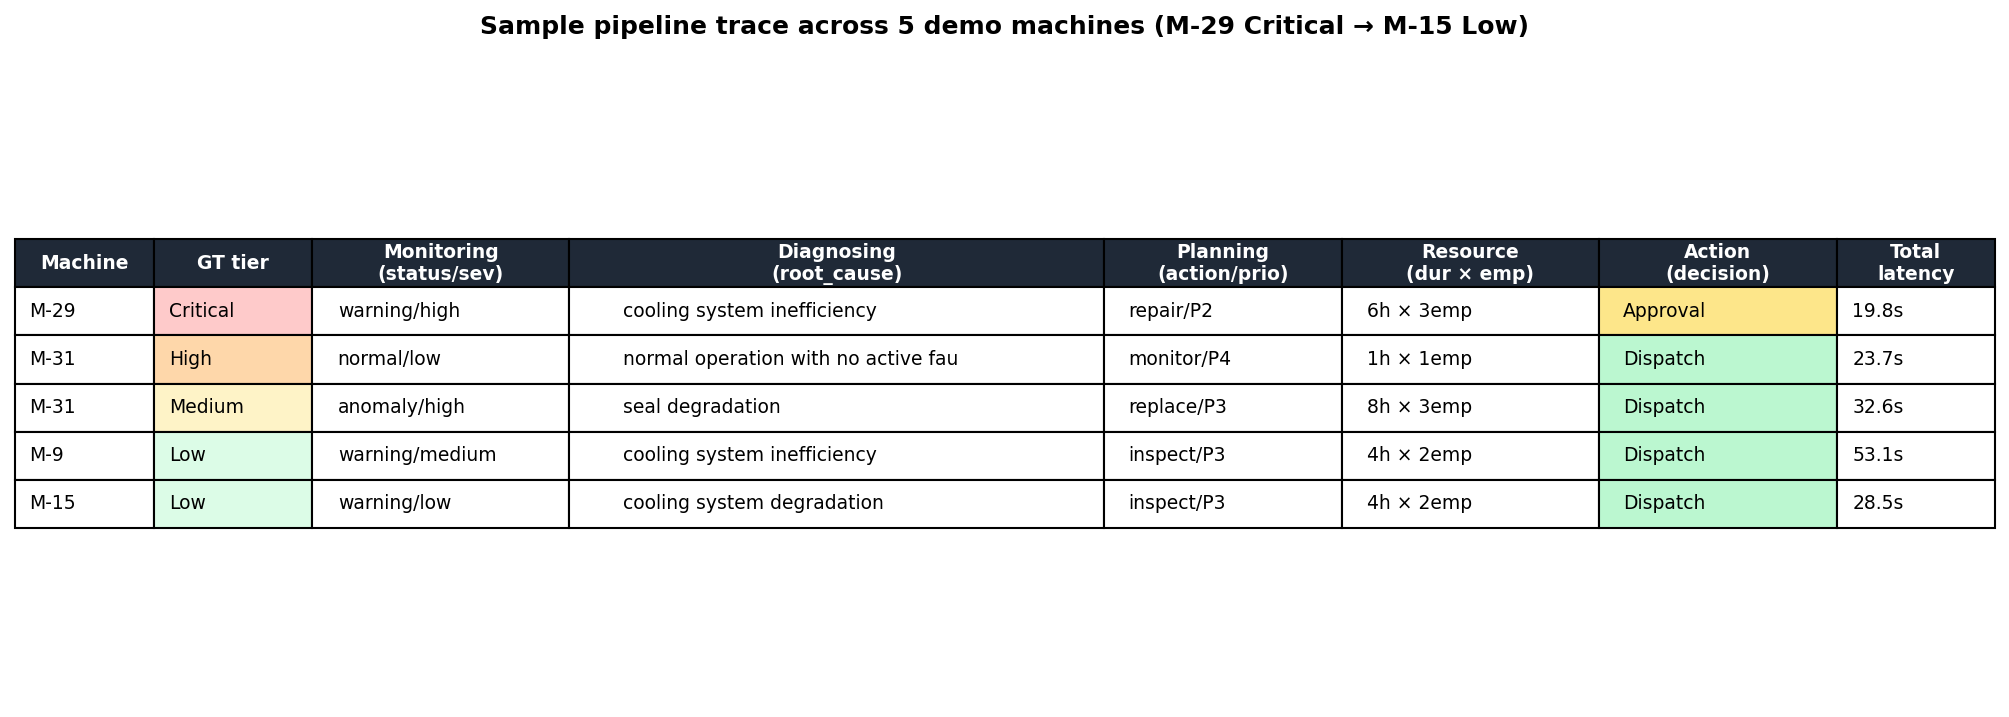
\includegraphics[width=\textwidth]{figures/trace_table.png}
    \caption{Sample pipeline trace across 5 demo machines. The Critical machine (M-29, RUL = 7~h) is correctly routed to a P2 repair action requiring supervisor approval; the misclassified High-tier machine (M-31, anomaly\_flag = 0 but RUL = 10~h) was assessed as normal by the Monitoring stage --- demonstrating both the strength (correct dispatch on clear cases) and a residual limitation (under-triage on edge-case High-tier where upstream classifier signals are mixed) of the sequential pipeline. Action column colour-coded: yellow = pending supervisor approval, green = automatic dispatch.}
    \label{fig:multi_agent_trace}
\end{figure}

\subsection{Per-Stage Latency Breakdown}

Figure~\ref{fig:multi_agent_latency} shows the per-stage wall-clock latency contribution per machine, with the 60-s Kafka producer cycle marked as a dashed reference line. Aggregate per-stage median / max latencies are:

\begin{table}[h!]
\centering
\caption{Multi-agent pipeline per-stage latency aggregates across 5 demo runs.}
\label{tab:multi_agent_latency}
\begin{tabular}{lllrr}
\hline
\textbf{Stage} & \textbf{Role} & \textbf{LLM} & \textbf{Median (s)} & \textbf{Max (s)} \\
\hline
1 & Monitoring & \texttt{glm-5.1:cloud} & 6.2 & 13.3 \\
2 & Diagnosing & \texttt{deepseek-v4-pro:cloud} & 10.2 & 40.4 \\
3 & Planning & \texttt{kimi-k2.6:cloud} & 3.2 & 4.1 \\
4 & Action & \texttt{deepseek-v4-pro:cloud} & 4.5 & 13.3 \\
\hline
\textbf{Total per case} & --- & --- & \textbf{28.5} & \textbf{53.1} \\
\hline
\end{tabular}
\end{table}

\begin{figure}[htbp]
    \centering
    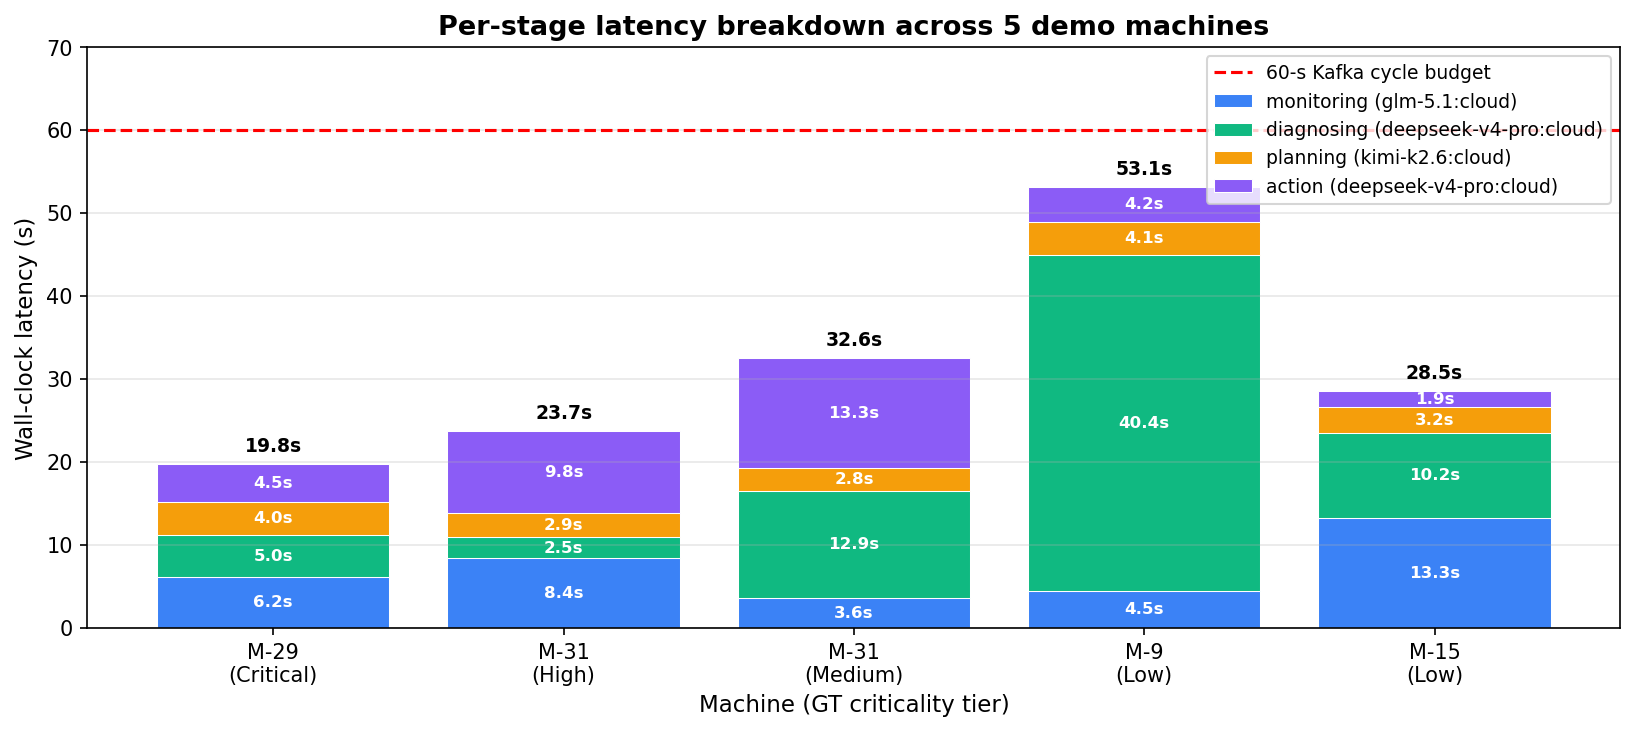
\includegraphics[width=\textwidth]{figures/latency_breakdown.png}
    \caption{Per-stage wall-clock latency breakdown across 5 demo machines. The dashed red line marks the 60-s Kafka producer cycle budget. All 5 pipelines complete within budget; the maximum (M-9 at 53.1~s, dominated by a 40.4~s Diagnosing call on the slowest LLM-API round-trip) leaves only 7-s margin and represents the worst-case scenario observed across the demo set.}
    \label{fig:multi_agent_latency}
\end{figure}

\subsection{Comparison to E-L2 V3 Ensemble}

The sequential 4-stage pipeline and the parallel V3 ensemble (preceding section) are complementary deployment patterns, not competing solutions. The trade-offs are summarised in Table~\ref{tab:multi_agent_vs_ensemble}.

\begin{table}[h!]
\centering
\caption{Sequential 4-stage pipeline vs parallel V3 ensemble.}
\label{tab:multi_agent_vs_ensemble}
\begin{tabular}{p{4cm}p{4.5cm}p{5cm}}
\hline
\textbf{Aspect} & \textbf{V3 Ensemble (preceding section)} & \textbf{4-Stage Pipeline (this section)} \\
\hline
LLM topology & 3 LLMs in parallel & 4 stages, each one LLM (sequential) \\
Output & Single tier label per machine & Full audit trail: monitoring + diagnosis + plan + dispatch \\
Latency p95 & 32.7 s & 53.1 s (worst case observed) \\
Empirical validation & $\kappa = 0.7425$ vs composite GT (N = 125) & Demo on 5 machines (illustrative, not statistically validated) \\
Failure mode tolerance & Majority vote allows one LLM to fail & Sequential halt: any stage parse-failure stops the pipeline \\
Use case fit & Real-time tier classification at scale & Case-level audit requirements (regulated industries, post-incident review) \\
\hline
\end{tabular}
\end{table}

The two patterns can also be \emph{composed}: the parallel ensemble produces the tier classification at high throughput and confidence, and the sequential pipeline is invoked only on machines flagged Critical (or for a sample audit) to produce the structured audit trail. This compositional usage avoids the latency cost of the sequential pipeline on Low/Medium-tier machines (the majority of fleet activity) while preserving full auditability where it matters most.

\subsection{Honest Scope and Limitations}

The 4-stage pipeline demonstration in this section is \emph{illustrative}, not statistically validated. Five machines do not constitute a sample sufficient to claim quantitative reliability of the diagnostic root-cause field, the planning action choice, or the dispatch decision quality. The substantive empirical validation of Layer~2 in this thesis is the V3 ensemble result ($\kappa = 0.7425$) reported in the preceding section.

The pipeline does demonstrate several deployment-relevant properties on this small sample: (a) all 5 runs completed all 4 stages without parse failure; (b) the Critical-tier machine was correctly routed to a high-priority repair action requiring supervisor approval; (c) the human-in-the-loop approval gate fired correctly only for P2-priority actions; (d) end-to-end latency stayed within the 60-s real-time budget on all 5 cases (worst case 53.1~s, 7-s margin). Validation at fleet scale across multiple seeds and human-rater agreement on diagnostic and planning outputs is reserved as future work.
